% Part: sets-functions-relations
% Chapter: relations
% Section: trees

\documentclass[../../../include/open-logic-section]{subfiles}

\begin{document}

\olfileid{sfr}{rel}{tre}
\olsection{Wit}

Jinis tatanan parsial tartamtu kang nduweni peran wigati
ing kabeh perangan logika yaiku \emph{wit}.
Wit winates katon ing perangan dhasar logika:
tuladhane, !!{formula}s bisa dingerteni lumantar
panguraiane dadi wit sintaksis, dene !!{derivation}s
ing akeh sistem !!{derivation} uga awujud wit winates.
%
Wit tanpa wates wis katon ing bukti teorema-teorema
kelengkapan kanggo logika proposisional lan logika
tataran kapisan, lan digunakake ing saindenging logika matematis.

Konsep wit ing teori himpunan raket gayutane karo
gagasan wit ing teori graf.
Iki gambar sawijining wit (winates):

\begin{center}
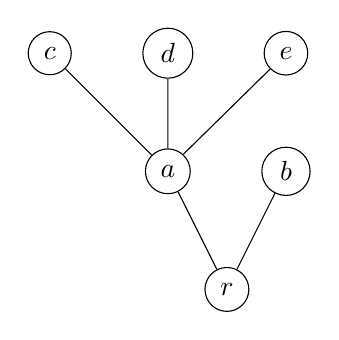
\begin{tikzpicture}[nodes={draw, circle}, -]
\node{$r$} [grow'=up]
    child { node {$a$}
        child { node {$c$} }
        child { node {$d$} }
        child { node {$e$} }
    }
    child { node {$b$} };
\end{tikzpicture}
\end{center}

Simpul paling ngisor~$r$ iku oyod.
Saben simpul saliyane $r$ duwe persis siji simpul induk
langsung ing sangisore. Kita bisa nganggep relasi
kang diduweni simpul~$x$ marang simpul~$y$ yen
$y$ bisa digayuh saka~$x$ kanthi ngetutake rusuk
munggah, minangka $x$ dadi \emph{leluhur} saka~$y$.

Relasi leluhur ing wit iku tatanan parsial ketat.
Iki dadi dhasar definisi miturut teori himpunan.
Kanggo nyatakake, kita mbutuhake rong konsep.
\emph{Anggota paling cilik} ing himpunan~$A$
kang ditata parsial dening~$\le$ yaiku
!!a{element} $x \in A$ kang ndadekake
kanggo kabeh $y \in A$ kita duwe~$x \le y$.
Himpunan \emph{katata kanthi becik} dening~$\le$
yen saben subhimpunane kang ora kosong duwe
anggota paling cilik.

\begin{defn}[Wit]
\emph{Wit} yaiku pasangan $T = \tuple{A, \le}$
kang ndadekake $A$ iku himpunan lan $\le$
iku tatanan parsial ing~$A$ kanthi siji-sijine
anggota paling cilik $r \in A$
(diarani \emph{oyod}), lan kanggo kabeh $x \in A$,
himpunan $\Setabs{y}{y \le x}$
katata kanthi becik dening~$\le$.
\end{defn}

\begin{defn}[Panerus]
Umpamakna $T = \tuple{A, \le}$ iku wit.
Yen $x,y \in A$, $x < y$, lan ora ana
$z \in A$ kang ndadekake $x < z < y$,
mula kita nyebut $y$ minangka \emph{panerus} saka~$x$.
\end{defn}

Panerus-panerus saka $x \in A$ uga diarani \emph{anake}.
Yen $y$ iku panerus saka~$x$, mula kita nyebut $x$
minangka \emph{pandhisik} utawa \emph{induk} saka~$y$.

\begin{prop}
Yen $\tuple{A,\le}$ iku wit, mula saben $x \in A$
saliyane oyod duwe paling akeh siji pandhisik.
\end{prop}

\begin{proof}
  Umpamakna $y_1 < x$, $y_2 < x$, lan $y_1 \neq y_2$.
  Mula $\{y_1,y_2\} \subseteq \Setabs{z}{z<x}$.
  Amarga $\Setabs{z}{z<x}$ katata kanthi becik
  dening~$\le$, subhimpunane $\{y_1, y_2\}$
  duwe anggota paling cilik, kang mesthi
  $y_1$ utawa~$y_2$.
  Mula $y_1 \le y_2$ utawa $y_2 \le y_1$.
  Kita nganggep $y_1 \neq y_2$, mula sejatine
  $y_1 < y_2$ utawa $y_2 < y_1$.
  Amarga kita nganggep $y_1 < x$ lan $y_2 < x$,
  kita uga duwe $y_1 < y_2< x$ utawa
  $y_2 < y_1 < x$.
  Mula $y_1$ lan $y_2$ ora bisa loro-lorone
  dadi pandhisik saka~$x$.
\end{proof}

\begin{defn}
Wit $T = \tuple{A, \le}$ diarani \emph{tanpa wates}
yen $A$ iku himpunan tanpa wates, lan
\emph{winates} yen ora mangkono.
Yen $T$ nduweni sipat saben $x \in A$
mung duwe panerus kang cacahe winates,
mula kita nyebut $T$ \emph{winates cacah paneruse ing saben simpul}.
\end{defn}

\begin{defn}[Pang]
Kanggo wit $T = \tuple{A, \le}$, \emph{pang} saka~$T$
yaiku rantai maksimal ing~$T$, yaiku himpunan
$B \subseteq A$ kang ndadekake kanggo saben
$x, y \in B$, $x \le y$ utawa $y \le x$,
lan kanggo saben $z \in X \setminus B$
ana $u \in B$ kang ndadekake
ora $z \le u$ lan ora $u \le z$.
%
Kita nganggo $[T]$ kanggo nglambangake
himpunan kabeh pang saka $T$.
\end{defn}

\begin{ex}
Tuladha klasik wit kang winates cacah paneruse ing saben simpul yaiku
\emph{wit biner tanpa wates} saka urutan winates
kang ngemot $0$ lan~$1$, kadhangkala
dilambangake $\{0,1\}^*$ utawa~$\Bin^*$,
ditata nganggo relasi ekstensi $\sqsubseteq$
(tuladhane, $101 \sqsubseteq 101101$).
Amarga saben rerangken biner tansah bisa
ditambahi $0$ utawa $1$ ing pungkasane,
wit iki ngemot anggota kang cacahe tanpa wates:
saben anggota~$s$ duwe persis rong panerus,
$s0$ lan~$s1$.
Oyode yaiku urutan kosong $\emptyseq$.
\end{ex}

\begin{ex}
Kanthi rada luwih umum, himpunan urutan winates
wilangan natural~$\Nat^*$ kanthi relasi
ekstensi~$\sqsubseteq$ uga wit.
Cetha yen wit iki ora winates cacah paneruse ing saben simpul:
saben $s \in \Nat^*$ duwe panerus~$sn$
kang cacahe tanpa wates, siji kanggo saben
$n \in \Nat$.
Saben $A\subseteq \Nat^*$ kang katutup
tumrap~$\sqsubseteq$ iku \emph{subwit}
saka~$\Nat^*$.
(Yaiku, $A$ nduweni sipat yen $s \in A$
lan $s' \sqsubseteq s$, mula uga $s' \in A$.)
Kabeh wit winates bisa diwakili minangka
subwit winates saka~$\Nat^*$.
\end{ex}

\begin{prop}[Lema K\H{o}nig]
Yen $T = \tuple{A,\le}$ iku wit tanpa wates
kang winates cacah paneruse ing saben simpul, mula $T$
duwe pang tanpa wates.
\end{prop}

Kasus khusus lema K\H{o}nig kang akeh digunakake
ing teori komputabilitas, dikenal minangka
\emph{lema K\H{o}nig ringkih}, yaiku mangkene:
saben subwit tanpa wates saka $\{0,1\}^*$
duwe pang tanpa wates.

\end{document}
